\chapter{METODE PENELITIAN}

\section{Tahapan Penelitian}

Tahapan dalam penelitian ini dapat dilihat pada gambar \ref{pict}

\begin{figure}[H]
    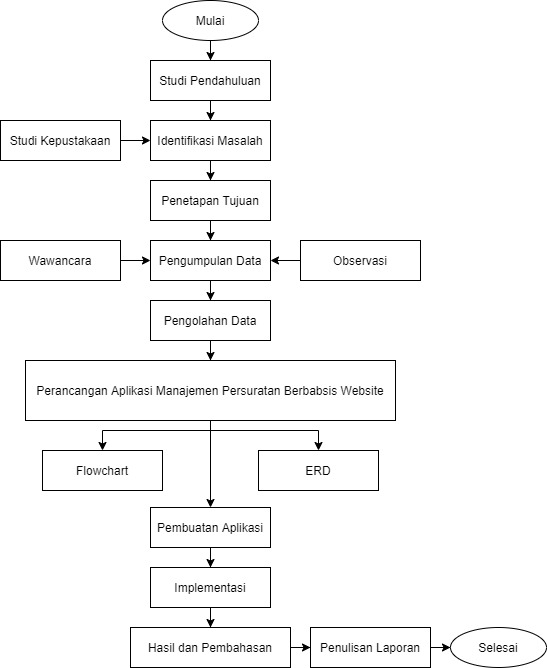
\includegraphics[width=0.8\linewidth, center]{images/flowchart-penelitian.jpg}
    \caption{Flowchart Tahapan Penelitian}
    \label{pict}
\end{figure}

Dalam perancangan Aplikasi Manajemen Persuratan ini, maka peneliti akan memperjelas tahapan-tahapan yang dilakukan dari mulai penelitian hingga selesai.

\subsection{Studi Pendahuluan}

Studi Pendahuluan merupakan bagian awal dari penelitian yang bertujuan untuk mendapatkan masukan yang diperlukan sehingga dapat menjadi dasar pembuatan aplikasi yang lebih baik serta dapat menyempurnakan penelitian ini. Hal ini dilakukan dengan kegiatan membaca beberapa referensi yang berkaitan dengan permasalahan yang sedang diteliti, dalam hal ini manajemen persuratan berbasis \textit{Website}.

\subsection{Studi Kepustakaan}

Studi Kepustakaan yaitu mencari teori-teori yang telah berkembang dalam bidang ilmu yang berpengaruh dalam penelitian ini dan mencari metode teknik penelitian, baik dalam pengumpulan data pengolahan dan menganalisa data.

\subsection{Identifikasi Masalah}

Identifikasi Masalah yaitu masalah-masalah yang mungkin timbul pada penelitian ini, dalam hal ini masalah yang ditemukan adalah kurang efisiennya sistem manajemen persuratan yang digunakan karena masih menggunakan sistem yang manual. Oleh sebab itu untuk mengatasi permasalahan yang ada, dibutuhkan suatu sistem informasi yang dapat memanajemen surat menjadi lebih baik.

\subsection{Penetapan Tujuan}

Penetapan Tujuan yaitu hasil yang ingin dicapai setelah pembuatan Aplikasi Manajemen Persuratan.

\subsection{Pengumpulan Data}

Pengumpulan Data merupakan tahap pengambilan data atau sampel yang berhubungan dengan permasalahan yang sedang dibahas, akan dibuat rancangan sistem informasinya dan selanjutnya dibuat aplikasi manajemen persuratannya. Dalam pengumpulan data tersebut menggunakan teknik-teknik pengumpulan data, yaitu :

\begin{enumerate} [label=\textbf{\alph*.}]

    \item \textbf{Wawancara} \\ 
    Wawancara yaitu proses memperoleh keterangan untuk tujuan penelitian dengan cara tanya jawab dengan pihak Kantor Desa Lampenai yang berkaitan dengan permasalahan yang sedang diteliti.
    \item \textbf{Observasi} \\
    Observasi yaitu pengumpulan data dengan mengadakan peninjauan langsung terhadap sistem yang sedang berlaku sehingga kita mendapatkan data yang aktual dari hasil penelitian yang dilakukan.
    
\end{enumerate}